% Copyright (C) Data Structures and Algorithms Team.
\chapter{Sets}
A set contains a number of values, the values are in no particular order and the values within the set are distinct from one another.

Generally set implementations tend to check that a value is not in the set first, before adding it to the set and so the issue of repeated values within the set is not an issue.

This section does not cover set theory in depth, rather it demonstrates briefly the ways in which the values of sets can be defined, and common operations that may be performed upon them.

The following $A = \{4, 7, 9, 12, 0\}$ defines a set $A$ whose values are listed within the curly braces. 

Given the set $A$ defined previously we can say that $4$ is a member of $A$ denoted by $4 \in A$, and that $99$ is not a member of $A$ denoted by $99 \notin A$.

Often defining a set by manually stating its members is tiresome, and more importantly the set may contain a large amount of values. A more concise way of defining a set and its members is by providing a series of properties that the values of the set must satisfy. In the following $A = \{x|x > 0, x~\%~2 = 0\}$ the set $A$ contains only positive integers that are even, $x$ is an alias to the current value we are inspecting and to the right hand side of $\mid$ are the properties that $x$ must satisfy to be in the set $A$ that is it must be $> 0$, and the remainder of the arithmetic expression $x / 2$ must be $0$.
You will be able to note from previous definition of the set $A$ that the set can contain an infinite number of values, and that the values of the set $A$ will be all even integers that are a member of the natural numbers set $\mathbb{N}$, where $\mathbb{N} = \{1, 2, 3, ...\}$.

Finally in this brief introduction to sets we will cover set intersection and union, both of which are very common operations (amongst many others) performed on sets. The union set can be defined as follows $A \cup B = \{x \mid x \in A~or~x \in B\}$, and intersection $A \cap B = \{x \mid x \in A~and~x \in B\}$. Figure \ref{fig:set_intersection_and_union} demonstrates set intersection and union graphically.

\begin{figure}
\begin{center}
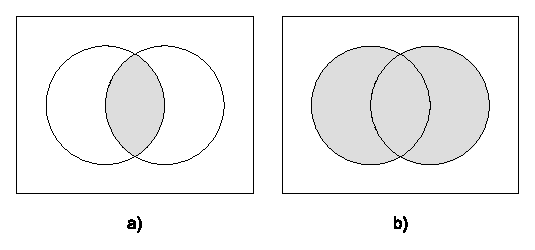
\includegraphics{set_intersection_and_union}
\end{center}
\caption{a) $A \cap B$; b) $A \cup B$} \label{fig:set_intersection_and_union}
\end{figure} 

Given the following set definitions $A = \{1, 2, 3\}$, and $B = \{6, 2, 9\}$ the union of the two sets is $A \cup B= \{1, 2, 3, 6, 9\}$, and the intersection of the two sets is $A \cap B= \{2\}$.

Both set union and intersection are sometimes provided within the framework associated with mainstream languages, this is the case in .NET 3.5\footnote{\url{http://www.microsoft.com/NET/}} where such algorithms exist as extension methods defined in the type \textit{System.Linq.Enumerable}\footnote{\url{http://msdn.microsoft.com/en-us/library/system.linq.enumerable_members.aspx}}, as a result DSA does not provide implementations of these algorithms.

\section{Unordered}
Sets in the general sense do not enforce the explicit ordering of their members, for example the members of $B = \{6, 2, 9\}$ conform to no ordering scheme because it is not required. 

Most libraries provide implementations of unordered sets and so DSA does not, we simply mention it here to disambiguate between an unordered set and ordered set. 

We will only look at insertion for an unordered set and cover briefly why a hash table is an efficient data structure to use for its implementation.

\subsection{Insertion}
Unordered sets can be efficiently implemented using a hash table as its backing data structure. As mentioned previously we only add an item to a set if that item is not already in the set, thus the backing data structure we use must have a quick look up and insertion run time complexity.

A hash map generally provides the following:

\begin{enumerate}
\item $O(1)$ for insertion
\item approaching $O(1)$ for look up
\end{enumerate}

The above depends on how good the hashing algorithm of the hash table is, however most hash tables employ incredibly efficient general purpose hashing algorithms and so the run time complexities for the hash table in your library of choice should be very similar in terms of efficiency.

\section{Ordered}
An ordered set is similar to an unordered set in the sense that its members are distinct, however an ordered set enforces some predefined comparison on each of its members to result in a set whose members are ordered appropriately.

In DSA 0.5 and earlier we used a binary search tree (defined in \S\ref{bst}) as the internal backing data structure for our ordered set, from versions 0.6 onwards we replaced the binary search tree with an AVL tree primarily because AVL is balanced.

The ordered set has it's order realised by performing an inorder traversal upon its backing tree data structure which yields the correct ordered sequence of set members.

Because an ordered set in DSA is simply a wrapper for an AVL tree that additionally enforces the tree contains unique items you should read \S\ref{Avl} to learn more about the run time complexities associated with its operations.
